\documentclass[preview,tikz]{standalone}
\usepackage{subfig}
%\usepackage{xcolor}
\usetikzlibrary{circuits.logic.US,calc,arrows.meta,shapes.geometric,math,circuits.ee.IEC}

\definecolor{clock1}{HTML}{86E291}
\definecolor{clock2}{HTML}{FFA5FA}
\definecolor{clock3}{HTML}{00C8BC}
\definecolor{clock4}{HTML}{F2F2F2}
\definecolor{input}{HTML}{008DC8}
\definecolor{output}{HTML}{E28686}
\definecolor{fixed}{HTML}{000000}
\colorlet{cs1}{lightgray!20}
\colorlet{cs2}{lightgray!50}
\colorlet{cs3}{lightgray}
\colorlet{cs4}{gray}

\def\cellsize{0.425}
\tikzset{
  pics/cell/.style = {
    code = {%
      \coordinate (-center) at (0,0);
      \coordinate (-east) at (\cellsize, 0);
      \coordinate (-north) at (0, \cellsize);
      \coordinate (-west) at (-\cellsize, 0);
      \coordinate (-south) at (0, -\cellsize);
      
      \fill[draw=black, line width=0.2pt, rounded corners=0.3pt] (-west |- -south) rectangle (-east |- -north);
      \foreach \d in {-east, -north, -west, -south}
      \draw[black, line width=.2pt] ($(-center)!.7!45:(\d)$) circle[radius=.12];
    }
  },
  pics/via/.style={
    code={%
      \coordinate (-center) at (0,0);
      \coordinate (-east) at (\cellsize, 0);
      \coordinate (-north) at (0, \cellsize);
      \coordinate (-west) at (-\cellsize, 0);
      \coordinate (-south) at (0, -\cellsize);
      
      \fill[draw=black, line width=0.2pt, rounded corners=0.3pt] (-west |- -south) rectangle (-east |- -north);
      \draw[black, line width=0.2pt] (-center) circle [radius=0.32];
    }
  },
  pics/crossline/.style={
    code={%
      \coordinate (-center) at (0,0);
      \coordinate (-east) at (\cellsize, 0);
      \coordinate (-north) at (0, \cellsize);
      \coordinate (-west) at (-\cellsize, 0);
      \coordinate (-south) at (0, -\cellsize);
      
      \fill[draw=black, line width=0.2pt, rounded corners=0.3pt] (-west |- -south) rectangle (-east |- -north);
      \foreach \d in {-east, -north, -west, -south}
      \draw[black, line width=.2pt] (-center) -- ($(-center)!.9!45:(\d)$);
    }
  },
  pics/fixed/.style={
    code={%
      \coordinate (-center) at (0,0);
      \coordinate (-east) at (\cellsize, 0);
      \coordinate (-north) at (0, \cellsize);
      \coordinate (-west) at (-\cellsize, 0);
      \coordinate (-south) at (0, -\cellsize);
      
      \fill[draw=black, line width=0.2pt, rounded corners=0.3pt] (-west |- -south) rectangle (-east |- -north);
      \ifnum#1=0\relax
      \foreach \d in {-north, -south}
      \filldraw[white, line width=.2pt] ($(-center)!.7!45:(\d)$) circle[radius=.12];
      \else
      \foreach \d in {-east, -west}
      \filldraw[white, line width=.2pt] ($(-center)!.7!45:(\d)$) circle[radius=.12];
      \fi
    }
  },
}

\begin{document}

\begin{figure}
\centering
    \subfloat[circuit]{
    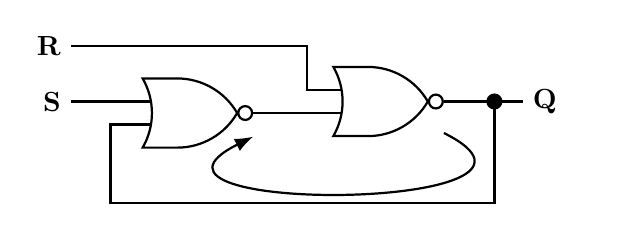
\begin{tikzpicture}[
    circuit logic US,
    circuit ee IEC,
    set make contact graphic= var make contact IEC graphic,
    huge circuit symbols,
    thick,
    ]
    \node at(3cm,0cm) [nor gate](nor1){};
    \draw (nor1.output) -- +(1cm,0cm) node[right](q){$\mathbf{Q}$};
    
    \node at([xshift=-2cm] nor1.input 2) [nor gate](nor2){};
    \draw(nor2.output) -- (nor1.input 2);
    
    \draw ([xshift=-1cm] nor2.input 1)node[left](s){$\mathbf{S}$} -- (nor2.input 1);
    \draw ([xshift=-1cm, yshift=0.7cm] nor2.input 1) node[left](r){$\mathbf{R}$} -- ++(3cm, 0) |- (nor1.input 1);
    
    \draw (nor2.input 2) -- ++(-0.5,0) -- ++(0,-1) -| ($(nor1.output)!.5!(q.center)$) node[contact]{};
    
    \draw[-{Latex}] ($(nor1.output)+(0,-0.4cm)$) .. controls +(2cm,-1cm) and  +(-2cm,-1cm) .. ($(nor2.output)+(0,-0.3cm)$);
    \end{tikzpicture}
    }
    \hfil
    \subfloat[layout]{
    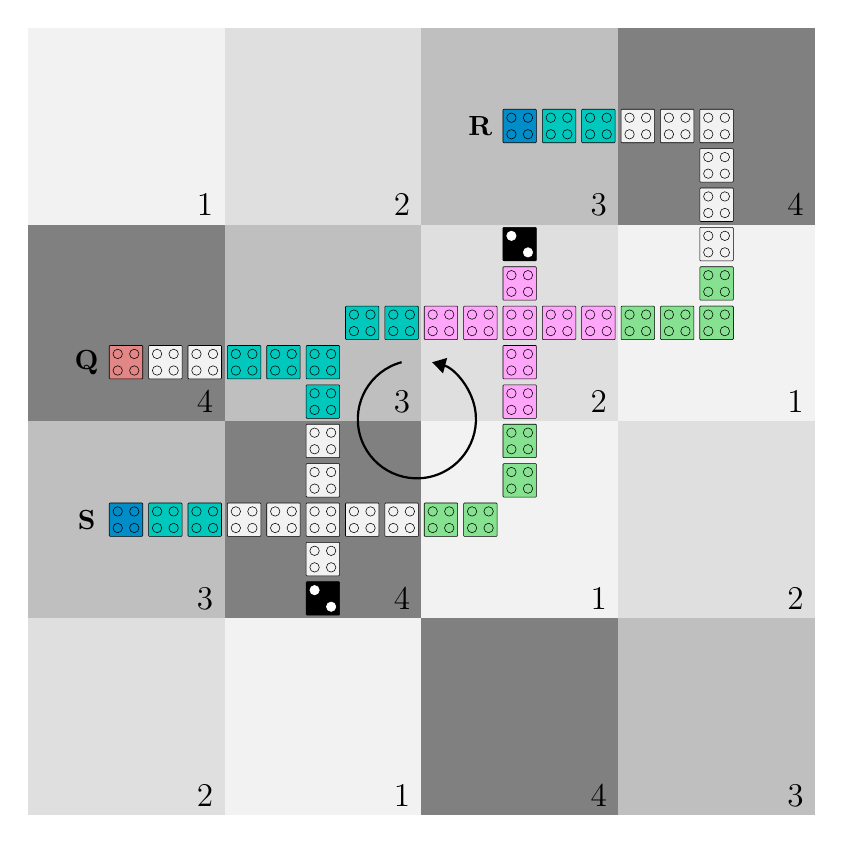
\begin{tikzpicture}[
      xscale=0.5,yscale=-0.5,
      ]
      \begin{scope}[
      x=5cm,y=5cm,
      shift={(2.5cm,2.5cm)},
      c1/.style={shape=rectangle, fill=cs1, text=black, minimum size=5cm},
      c2/.style={shape=rectangle, fill=cs2, text=black, minimum size=5cm},
      c3/.style={shape=rectangle, fill=cs3, text=black, minimum size=5cm},
      c4/.style={shape=rectangle, fill=cs4, text=black, minimum size=5cm},
      ]
        \tikzmath{
          function use(\x,\y){
            return (mod(\y,2)!=0) ? 
            ((mod(\y+1,4)!=0)?(4-mod(\x,4)):(4-mod(\x+2,4))) :
            ((mod(\y,4)==0)?(1+mod(\x,4)):(1+mod(\x+2,4)));
          };
          %
          int \i, \j, \c; 
          for \i in {0,1,2,3}{
            for \j in {0,1,2,3}{
              \c = use(\i,\j);
              {
                \path (\i,\j) 
                {[transform shape]node(\i\j)[c\c]{}} 
                ($(\i\j.center)!.8!(\i\j.north east)$) node{\large \c};
              };
            };
          };
        }
      \end{scope}
      
      \begin{scope}[
      shift={(0.4975cm,0.4975cm)},
      ]
      \begin{scope}[transform shape]
      \path
        (12,2) pic(r)[input]{cell} 
        (13,2) pic   [clock3]{cell}
        (14,2) pic   [clock3]{cell}
        (15,2) pic   [clock4]{cell}
        (16,2) pic   [clock4]{cell}
        (17,2) pic   [clock4]{cell}
      ;
      
      \path
        (8,7) pic[clock3]{cell}
        (9,7) pic[clock3]{cell}
        (10,7) pic[clock2]{cell}
        (11,7) pic[clock2]{cell}
        (12,7) pic[clock2]{cell}
        (13,7) pic[clock2]{cell}
        (14,7) pic[clock2]{cell}
        (15,7) pic[clock1]{cell}
        (16,7) pic[clock1]{cell}
        (17,7) pic[clock1]{cell}
      ;
      
      \path 
        (2,8) pic(q)[output]{cell}
        (3,8) pic   [clock4]{cell}
        (4,8) pic   [clock4]{cell}
        (5,8) pic   [clock3]{cell}
        (6,8) pic   [clock3]{cell}
        (7,8) pic   [clock3]{cell}
      ;
      
      \path 
        (2,12) pic(s)[input]{cell}
        (3,12) pic   [clock3]{cell}
        (4,12) pic   [clock3]{cell}
        (5,12) pic   [clock4]{cell}
        (6,12) pic   [clock4]{cell}
        (7,12) pic   [clock4]{cell}
        (8,12) pic   [clock4]{cell}
        (9,12) pic   [clock4]{cell}
        (10,12) pic   [clock1]{cell}
        (11,12) pic   [clock1]{cell}
      ;
      
      \path
        (7,9)  pic[clock3]{cell}
        (7,10) pic[clock4]{cell}
        (7,11) pic[clock4]{cell}
        (7,13) pic[clock4]{cell}
        (7,14) pic[fixed]{fixed=1}
      ;
      
      \path
        (12,5) pic[fixed]{fixed=1}
        (12,6) pic[clock2]{cell}
        (12,8) pic[clock2]{cell}
        (12,9) pic[clock2]{cell}
        (12,10) pic[clock1]{cell}
        (12,11) pic[clock1]{cell}
      ;
      
      \path
        (17,3) pic[clock4]{cell}
        (17,4) pic[clock4]{cell}
        (17,5) pic[clock4]{cell}
        (17,6) pic[clock1]{cell}
        (17,7) pic[clock1]{cell}
      ;
      
      \draw[-{Triangle},thick]
      % (9,8) .. controls +(-4,4) and +(4,4) .. (10,8);
      (9,8) arc[radius=1.5,start angle=255,end angle=-75];
      
      \end{scope}
      
      \node at (11,2){$\mathbf{R}$};
      \node at (1,12){$\mathbf{S}$};
      \node at (1,8) {$\mathbf{Q}$};
      \end{scope}
    \end{tikzpicture}
    }
\end{figure}
\end{document}
